\documentclass[11pt,letterpaper]{article}
\usepackage[top=2.0cm, bottom=3cm, left=2.0cm, right=2.0cm]{geometry}
\usepackage[utf8]{inputenc}
\usepackage[T1]{fontenc}
\usepackage[spanish]{varioref}
\usepackage[activeacute, spanish, es-tabla]{babel}
\usepackage{fancyhdr}
\usepackage{multicol}
\usepackage{float}
\usepackage{textcomp}
\usepackage{ae,aecompl}
\usepackage{amssymb,amsmath}
\usepackage[pdftex]{graphicx}
\usepackage{askmaps}
\usepackage{multirow}
\pagestyle{fancy} 
\pagenumbering{arabic} 
\renewcommand{\headrulewidth}{0pt} 
\setlength{\headsep}{20pt} 
\setlength{\headheight}{65pt} 
\setlength{\textheight}{600pt} 
\setlength{\columnsep}{15pt} 
\newcommand{\universidad}{\small{Universidad Técnica Federico Santa María}}
\newcommand{\campus}{\small{Campus Santiago San Joaquín}}

% Definiciones de Título e Integrantes de Experiencia
\newcommand{\titulo}{Informe Tarea 2 \\ Arquitectura y Organización de Computadores}
\newcommand{\integrantes}{\begin{tabular}{c}
Juan Pablo Jorquera  201573533-6 \\
Cristian Navarrete 201573549-2\\
\end{tabular}}

\renewcommand{\maketitle}
{
\thispagestyle{fancy}
\begin{center}
\begin{Large}
\textbf{\titulo}\\
\end{Large}
\end{center}
\vspace{0.3cm}
}


%ENCABEZADO

\fancyhead[R]{\begin{minipage}[b]{0.405\textwidth}
\begin{center}
\universidad \\ 
\campus \\ 
\integrantes
\end{center}
\end{minipage}}
\fancyhead[L]{\vspace{15pt}
\includegraphics[height=1.6cm]{Escudo.png}}
%%%%%%%%%%%%%%%%%%%%%%%%%%%%%%%%%%%%%%%%%%%%%%%%
%                                              %
% AQUI TERMINAN LAS DEFINICIONES DE ENCABEZADO %
% Y EMPIEZA EL CUERPO DEL DOCUMENTO            %
%                                              %
%%%%%%%%%%%%%%%%%%%%%%%%%%%%%%%%%%%%%%%%%%%%%%%%

\begin{document}
\setcounter{secnumdepth}{0}
\maketitle
Se busca realizar el circuito con las características requeridas, para ello en primer lugar realizamos el diagrama de estados correspondiente.

Se agregó en la etiqueta la parte de las secuencias que se va cumpliendo en cada estado (dígitos finales) para tener una mejor visualización.
\begin{center}
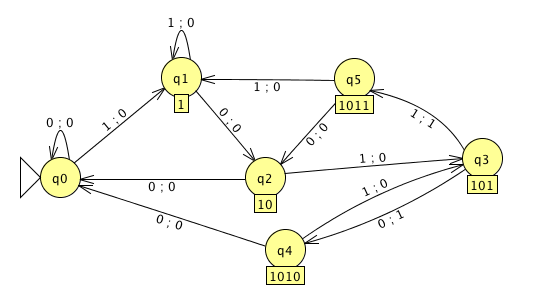
\includegraphics[width=15cm]{diag-estados.png}
\end{center}

Luego se enumeró arbitrariamente cada estado, como se muestra a continuación:
\vspace{0.2cm}
\begin{table}[h]
\centering
\begin{tabular}{c|c|c|c|}
\cline{2-4}
                             & \multicolumn{3}{c|}{Dígito} \\ \hline
\multicolumn{1}{|c|}{Estado} & A       & B       & C       \\ \hline
\multicolumn{1}{|c|}{$q_0$}     & 0       & 0       & 0       \\ \hline
\multicolumn{1}{|c|}{$q_1$}     & 0       & 0       & 1       \\ \hline
\multicolumn{1}{|c|}{$q_2$}     & 0       & 1       & 0       \\ \hline
\multicolumn{1}{|c|}{$q_3$}     & 0       & 1       & 1       \\ \hline
\multicolumn{1}{|c|}{$q_4$}     & 1       & 0       & 0       \\ \hline
\multicolumn{1}{|c|}{$q_5$}     & 1       & 0       & 1       \\ \hline
\end{tabular}
\end{table}

\newpage
Finalmente, con la enumeración de estados, se generó  la tabla de transición y de salida con la que se va a trabajar más adelante.
\begin{table}[h]
\centering
\caption{Tabla de Transición y Salida}
\vspace{0.2cm}
\label{tab_output}
\begin{tabular}{|l|c|c|c|c||l|c|c|c|c|}
\hline
\multicolumn{4}{|c|}{Estado}   & Input & \multicolumn{4}{l|}{Siguiente Estado} & Output \\ \hline
No.                & A & B & C & X      & No.       & D       & E      & F      &  Y      \\ \hline
\multirow{2}{*}{0} & 0 & 0 & 0 & 0     & 0         & 0       & 0      & 0      & 0      \\ \cline{2-10} 
                   & 0 & 0 & 0 & 1     & 1         & 0       & 0      & 1      & 0      \\ \hline
\multirow{2}{*}{1} & 0 & 0 & 1 & 0     & 2         & 0       & 1      & 0      & 0      \\ \cline{2-10} 
                   & 0 & 0 & 1 & 1     & 1         & 0       & 0      & 1      & 0      \\ \hline
\multirow{2}{*}{2} & 0 & 1 & 0 & 0     & 0         & 0       & 0      & 0      & 0      \\ \cline{2-10} 
                   & 0 & 1 & 0 & 1     & 3         & 0       & 1      & 1      & 0      \\ \hline
\multirow{2}{*}{3} & 0 & 1 & 1 & 0     & 4         & 1       & 0      & 0      & 1      \\ \cline{2-10} 
                   & 0 & 1 & 1 & 1     & 5         & 1       & 0      & 1      & 1      \\ \hline
\multirow{2}{*}{4} & 1 & 0 & 0 & 0     & 0         & 0       & 0      & 0      & 0      \\ \cline{2-10} 
                   & 1 & 0 & 0 & 1     & 3         & 0       & 1      & 1      & 0      \\ \hline
\multirow{2}{*}{5} & 1 & 0 & 1 & 0     & 2         & 0       & 1      & 0      & 0      \\ \cline{2-10} 
                   & 1 & 0 & 1 & 1     & 1         & 0       & 0      & 1      & 0      \\ \hline
\multirow{2}{*}{}  & 1 & 1 & 0 & 0     &           & X       & X      & X      & X      \\ \cline{2-10} 
                   & 1 & 1 & 0 & 1     &           & X       & X      & X      & X      \\ \hline
\multirow{2}{*}{}  & 1 & 1 & 1 & 0     &           & X       & X      & X      & X      \\ \cline{2-10} 
                   & 1 & 1 & 1 & 1     &           & X       & X      & X      & X      \\ \hline
\end{tabular}
\end{table}

A continuación se realizan los mapas de Karnaugh para cada salida correspondiente, usando la notación incluida en la tabla anterior.

\vspace{0.2cm}
\begin{center}
\askmap{4}{$D$}{{$A$}{$B$}{$C$}{$X$}}%
{000000110000XXXX}%
{%
\put(2,1){\oval(1.9,1.9)}
}
\askmap{4}{$E$}{{$A$}{$B$}{$C$}{$X$}}%
{001001000110XXXX}%
{%
\put(2,2.5){\oval(1.9,0.8)}
\put(3,2.5){\oval(1.9,0.7)}
\put(4,0.5){\oval(1.9,0.8)[l]}
\put(0,0.5){\oval(1.9,0.8)[r]}
}

\askmap{4}{$F$}{{$A$}{$B$}{$C$}{$X$}}%
{010101010101XXXX}%
{%
\put(2,2){\oval(3.9,1.8)}
}\askmap{4}{$Y$}{{$A$}{$B$}{$C$}{$X$}}%
{000000110000XXXX}%
{%
\put(2,1){\oval(1.8,1.8)}
}
\end{center}
\vspace{0.2cm}

Obteniendo así las siguientes funciones:
\begin{itemize}
	\item{$D = BC$}
	\item{$E = \overline{B}C\overline{X} + A\overline{C}X + B\overline{C}X$}
	\item{$F = X$}
	\item{$Y  = BC$}
\end{itemize}

\vspace{0.2cm}
\section{Extra}
Para ello se toman ambos inputs (la palabra y la clave), de ser necesario se deben transformar a binario, y se hacen pasar por un circuito sumador para que así el resultado sea el caracter codificado, es importante tener en cuenta que el Carry Out es lo que se debe ignorar para simplemente para emular el módulo que se realiza en el cifrado. Finalmente, como el resultado está en binario, bastaría transformar a hexadecimal de vuelta si así se requiere.


\end{document}
